\chapter{Experiments and Evaluation Framework}
\label{chp:experiments_and_framework}

This chapter defines what is being evaluated, how it is evaluated, and
what evidence the reader should expect in Chapter~\ref{chap:results}. It
is structured so that every experimental choice can be traced to a
concrete question and a concrete artefact in the repository.

Section~\ref{sec:rq_h} restates the research questions and derives
falsifiable hypotheses that Chapter~\ref{chap:results} will accept or
reject. Section~\ref{sec:train_test_split} defines the held-out
train/test split that separates discovery from evaluation.
Section~\ref{sec:process_discovery_methodology} describes the
control-flow discovery procedure and its conformance
protocol. Section~\ref{sec:simulation_discovery_methodology} defines
the three ProSiT configurations that will be compared:
distribution-based (no-rules), data-aware with decision trees
(rules) and data-aware with additional queue-length features
(rules$+$workload). Section~\ref{sec:mc_protocol} defines the
multi-seed Monte-Carlo replication protocol that produces the
confidence intervals used throughout Chapter~\ref{chap:results}.
Section~\ref{sec:evaluation_metrics} defines the fidelity metrics.
Section~\ref{sec:what_if_design} defines the two operational what-if
scenarios. Section~\ref{sec:results_percentile_sens_design} defines the
transition-baseline sensitivity study.
Section~\ref{sec:prosit_workarounds} documents the deviations from a
clean ProSiT invocation that were required to complete the experiments
on the CTB event log.

Figure~\ref{fig:research_design} gives an overview of the full
experimental pipeline. Every stage in the diagram is realised by a
script in the code repository; the section-level cross-references in
the caption identify the concrete implementation.

\begin{figure}[htbp]
\centering
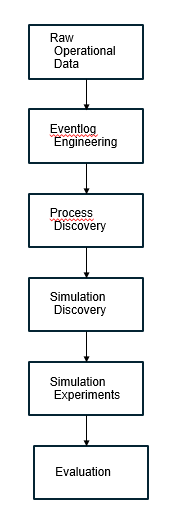
\includegraphics[width=0.95\textwidth]{figures/schemas/ResearchDesignV1.png}
\caption{Experimental pipeline. \emph{Data engineering} produces
\texttt{s6\_eventlog\_target\_rank\_features.csv} (Chapter~\ref{chp:case_study_and_data}).
The \emph{split} of Section~\ref{sec:train_test_split} separates the
log into training and held-out testing partitions. \emph{Process
discovery} (Section~\ref{sec:process_discovery_methodology}) yields the
Petri net used as the ProSiT skeleton. Three
\emph{simulation-parameter discovery} configurations
(Section~\ref{sec:simulation_discovery_methodology}) are compared;
each is evaluated against the held-out log through the
\emph{Monte-Carlo protocol} of Section~\ref{sec:mc_protocol}. Two
\emph{what-if} experiments (Section~\ref{sec:what_if_design}) exercise
the adopted-default configuration under operational disruption.}
\label{fig:research_design}
\end{figure}

%%%%%%%%%%%%%%%%%%%%%%%%%%%%%%%%%%%%%%%%%%%%%%%%%%%%%%%%%%%%%%%%%%%%%%%
\section{Research Questions, Hypotheses and Framing}
\label{sec:rq_h}
%%%%%%%%%%%%%%%%%%%%%%%%%%%%%%%%%%%%%%%%%%%%%%%%%%%%%%%%%%%%%%%%%%%%%%%

Chapter~\ref{chp:introduction} formulated the overarching research
questions. To make them empirically tractable, they are here refined
into testable claims. The claims deliberately admit rejection: an
outcome that contradicts a hypothesis is a valid contribution and is
reported as such in Chapter~\ref{chap:results}.

\subsection{Refined Research Questions}
\label{sec:refined_rq}

\begin{description}
\item[RQ1 (Fidelity).] To what extent does a ProSiT simulator
      discovered from historical CTB truck data reproduce case-level
      turnaround, activity durations, waiting times and arrivals on a
      held-out temporal test window?
\item[RQ2 (Structural quality).] Does the discovered Petri net
      generalise to the held-out period, or is fitness only preserved
      on the training period?
\item[RQ3 (Modelling choices).] How sensitive is simulation fidelity to
      three plausible ProSiT configurations
      (\textit{no-rules}, \textit{rules}, \textit{rules$+$workload})?
\item[RQ4 (Scenario support).] Does the discovered simulator produce
      operationally plausible KPI shifts under two transparent
      interventions: closing a single RMG block and increasing truck
      demand by 20\,\%?
\end{description}

\subsection{Hypotheses}
\label{sec:data_aware_hypotheses}

\begin{description}
\item[H1 (Time dependence of arrivals).] A time-aware arrival model
      (decision tree over hour, weekday, weekend indicator) reduces
      inter-arrival prediction error against a pooled-rate baseline on
      cross-validated hold-out slices from the training log.
\item[H2 (Data-aware fidelity gain).] Enabling ProSiT decision-tree
      rules (\textit{rules}) produces lower distributional distance to
      the held-out test log than the distribution-only ProSiT
      (\textit{no-rules}) for at least one of case-turnaround EMD,
      waiting-time EMD or service-time EMD.
\item[H3 (Workload-feature gain).] Adding queue-length and
      workload-history features to the ProSiT resource-selection and
      waiting-time models (\textit{rules$+$workload}) further reduces
      distributional distance versus \textit{rules} on the held-out
      test log.
\item[H4 (Scenario response).] Closing T22 eliminates assignments to
      that resource and increases RMG pre-service delay, while a
      20\,\% increase in working-time arrival intensity measurably
      increases the observed truck-arrival rate. Downstream
      turnaround effects are estimated rather than assumed.
\end{description}

Every hypothesis is intended to be falsifiable. In particular H2 and H3
are treated as claims of \emph{practical} benefit: the point estimate
must be lower and the 95\,\% confidence interval derived in
Section~\ref{sec:mc_protocol} must not overlap the reference configuration
entirely for the improvement to be reported as a fidelity gain.

%%%%%%%%%%%%%%%%%%%%%%%%%%%%%%%%%%%%%%%%%%%%%%%%%%%%%%%%%%%%%%%%%%%%%%%
\section{Held-Out Train/Test Split}
\label{sec:train_test_split}
%%%%%%%%%%%%%%%%%%%%%%%%%%%%%%%%%%%%%%%%%%%%%%%%%%%%%%%%%%%%%%%%%%%%%%%

\subsection{Rationale}

A held-out validation set is required to test H1--H3. In simulation
discovery it is not sufficient to report the fit of parameters on the
data used to discover them: a well-fit ProSiT bundle can memorise the
training distribution while over-fitting the operational dynamics. The
ProSiT reference implementation \cite{Vinci2026prosit} describes an
in-memory split in its \textit{Advanced Usage} example, but does not
persist the split, does not commit to a case-level boundary and does
not report validation metrics. This thesis therefore uses a persistent,
case-level, temporally ordered split that any downstream script can
consume unchanged.

\subsection{Split Definition}
\label{sec:split_definition}

Let $\mathcal{L}=(c_1,c_2,\dots,c_N)$ be the set of $N=89{,}460$ cases
in the final event log. For each case $c_i$ let $\tau(c_i)$ denote its
earliest event timestamp:
\begin{equation}
    \tau(c_i)=\min\bigl\{
      \text{start}(e),\text{time}(e)
      \mid e\in c_i \bigr\}.
\end{equation}
Sort the cases by $\tau$ and a deterministic case-identifier
tiebreaker. The first 80\,\% form the training set and the remaining
20\,\% form the test set. The cutoff $\tau^{\star}$ is recorded as the
earliest arrival in the test set. Cases whose earliest event timestamp
is missing are dropped from both.

On the CTB event log the cutoff is
$\tau^{\star}=\text{2026-04-20 18:17:00}$. The split produces 71,568
training cases (220,048 events) and 17,892 testing cases (55,360
events); no events are dropped. The split is realised by
\texttt{validation/01\_train\_test\_split.py} and is documented in
\texttt{validation/results/split\_manifest.json}, which also records
the seed, the cutoff and the per-activity coverage in both partitions.
The manifest is loaded by every downstream simulation script so that
$n_{\text{traces}}$ and $t_{\text{start}}$ match the test window
exactly.

\subsection{Correction Relative to Earlier Drafts}

Earlier versions of this thesis referenced a training set of 24,000
cases and a test set of 6,000 cases. Those numbers were an artefact of
a legacy random-subsample step in
\texttt{baseline/export\_empirical\_durations.py} that only fired when
the discovery scripts were pointed at the full event log. All discovery
scripts are now routed through
\texttt{baseline/\_eventlog\_source.py}, which prefers the persisted
\texttt{s6\_train.csv} and skips the legacy subsample when a train log
is detected. The correct partitioning is therefore 71,568/17,892 as
recorded in the split manifest.

%%%%%%%%%%%%%%%%%%%%%%%%%%%%%%%%%%%%%%%%%%%%%%%%%%%%%%%%%%%%%%%%%%%%%%%
\section{Process Discovery Protocol}
\label{sec:process_discovery_methodology}
%%%%%%%%%%%%%%%%%%%%%%%%%%%%%%%%%%%%%%%%%%%%%%%%%%%%%%%%%%%%%%%%%%%%%%%

\subsection{Algorithm}

The Petri net that ProSiT uses as the authoritative control-flow
skeleton is constructed from the observed training variants as a
sequential prefix trie. Every accepted path has the form
\texttt{Gate In}$\rightarrow$one or more yard activities
$\rightarrow$\texttt{Gate Out}. Shared prefixes are represented once,
and a separate transition encodes each observed continuation. This
prevents an inductive-miner concurrency cut from enabling two yard
activities inside the same truck visit. It does \emph{not} disable
multitasking between trucks: different cases still compete for and can
use resources concurrently according to the discovered capacities.

An inductive process tree is retained as a diagnostic visualisation,
but it is not passed to the final simulator. The authoritative trie is
implemented by \texttt{\_eventlog\_contract.py} and injected by
\texttt{baseline/07\_run\_prosit\_discovery.py}. It contains 76 places
and 144 transitions for the 70 variants observed in the frozen training
partition.

\subsection{Conformance Protocol}

Control-flow conformance metrics are computed against
\emph{both} the training and the held-out testing partition:

\begin{itemize}
    \item Token-based replay \textbf{fitness}, i.e.\ the fraction of
          traces that the Petri net can replay without token deficit.
    \item Token-based replay \textbf{precision}, the share of behaviour
          allowed by the model that is also observed in the log.
    \item \textbf{Generalisation} via
          \texttt{pm4py.generalization\_tbr}.
    \item \textbf{Simplicity} via \texttt{pm4py.simplicity\_petri\_net}.
\end{itemize}

They are supplemented by an explicit case-language audit: exactly one
initial Gate In, at least one yard activity, exactly one final Gate Out,
no within-case activity overlap and monotonically non-decreasing
completion timestamps. This separates two questions that aggregate
fitness alone cannot answer: whether the net replays held-out variants
and whether the generated traces obey the physical truck-visit order.
The full protocol is implemented in
\texttt{baseline/07\_run\_prosit\_discovery.py} and
\texttt{\_eventlog\_contract.py}.

%%%%%%%%%%%%%%%%%%%%%%%%%%%%%%%%%%%%%%%%%%%%%%%%%%%%%%%%%%%%%%%%%%%%%%%
\section{Simulation Parameter Discovery Configurations}
\label{sec:simulation_discovery_methodology}
%%%%%%%%%%%%%%%%%%%%%%%%%%%%%%%%%%%%%%%%%%%%%%%%%%%%%%%%%%%%%%%%%%%%%%%

ProSiT is used unchanged as the discovery and simulation engine
\cite{Vinci2026prosit}. All simulation parameters are learned by
\texttt{SimulatorParameters.discover\_from\_eventlog} from the training
partition only. Three configurations are evaluated. They are chosen so
that H2 (data-aware fidelity gain) and H3 (workload-feature gain) each
correspond to exactly one comparison.

\subsection{Configuration \textit{no-rules}}
\label{sec:cfg_no_rules}

The \textit{no-rules} configuration uses
\texttt{max\_depth\_tree}$=0$, which disables the ProSiT decision-tree
mechanism entirely. Every parameter reduces to a single unconditional
distribution or a marginal frequency: one arrival-rate distribution,
one execution-time distribution per activity, one waiting-time
distribution per resource, one categorical distribution over routing
choices at each Petri-net decision point. This configuration is the
distribution-based baseline against which H2 is tested.

\subsection{Configuration \textit{rules}}
\label{sec:cfg_rules}

The \textit{rules} configuration uses the ProSiT default
(\texttt{max\_depth\_tree}$=3$,
\texttt{min\_samples\_leaf\_cv}$=[50,100,200]$,
\texttt{random\_state}$=42$). Every timing, routing and
resource-selection model is fitted as a decision tree whose leaves
carry the local distributions. Cross-validation over the leaf-size grid
selects the actual leaf size per model, and models that fail to beat
the marginal distribution on held-out CRPS collapse to the pooled
baseline (this is a ProSiT internal safeguard against overfitting to
noise \cite{Vinci2026prosit}). Case-level attributes made available to
the trees are the container, demand, utilisation, target-area and
temporal features listed in
Section~\ref{sec:eventlog_structure}.

\subsection{Configuration \textit{rules$+$workload}}
\label{sec:cfg_workload}

The \textit{rules$+$workload} configuration is identical to
\textit{rules} but with
\texttt{use\_workload\_features}$=$\texttt{True}. As documented in the
ProSiT README this enables two extra features on the waiting-time and
resource-selection models: current workload (number of concurrent
tasks) and queue length (number of tasks scheduled but not yet started)
at the time each event is enabled in the process model. The intention behind including this
configuration is to let ProSiT see the queueing state that its
distribution family alone would otherwise ignore. This configuration is
compared against \textit{rules} to test H3.

\subsection{Discovery Hyperparameters}

Table~\ref{tab:prosit_hyperparams} lists the ProSiT hyperparameters
that differ across configurations. All other arguments are the ProSiT
defaults except \texttt{attribute\_mode}, which is set to
\texttt{'empirical'} for reasons detailed in
Section~\ref{sec:prosit_workarounds}.

\begin{table}[h]
\centering
\caption{ProSiT discovery hyperparameters by configuration.}
\label{tab:prosit_hyperparams}
\begin{tabular}{lccc}
\toprule
\textbf{Hyperparameter} & \textbf{no-rules} & \textbf{rules} & \textbf{rules$+$workload} \\
\midrule
\texttt{max\_depth\_tree}          & 0             & 3             & 3 \\
\texttt{min\_samples\_leaf\_cv}    & --            & [50, 100, 200] & [50, 100, 200] \\
\texttt{use\_workload\_features}   & False         & False         & True \\
\texttt{attribute\_mode}           & \texttt{empirical} & \texttt{empirical} & \texttt{empirical} \\
\texttt{random\_state}             & 42            & 42            & 42 \\
\bottomrule
\end{tabular}
\end{table}

The full pipeline is executed by
\texttt{baseline/07\_run\_prosit\_discovery.py}. The pickled
\texttt{SimulatorParameters} objects
(\texttt{prosit\_params.pkl}) and their JSON representations are stored
in the paramset folder
\path{baseline/discovery_params/params_<utc>_train80/prosit_discovery_no_rules|_workload|/}.

%%%%%%%%%%%%%%%%%%%%%%%%%%%%%%%%%%%%%%%%%%%%%%%%%%%%%%%%%%%%%%%%%%%%%%%
\section{Monte-Carlo Replication Protocol}
\label{sec:mc_protocol}
%%%%%%%%%%%%%%%%%%%%%%%%%%%%%%%%%%%%%%%%%%%%%%%%%%%%%%%%%%%%%%%%%%%%%%%

Every ProSiT simulation includes stochastic draws from the fitted
distributions. Reporting a single Monte-Carlo draw is therefore
insufficient to conclude that one configuration is more faithful than
another: the observed difference may be within the sampling variance
of the simulator itself. This thesis therefore reports every fidelity
metric with a Monte-Carlo confidence interval.

\subsection{Replication Design}

For each ProSiT configuration
$\text{cfg}\in\{\textit{no-rules},\textit{rules},\textit{rules$+$workload}\}$
the following procedure is executed:

\begin{enumerate}
    \item Load the corresponding \texttt{SimulatorParameters} bundle
          from disk.
    \item Instantiate a fresh \texttt{SimulatorEngine}.
    \item For $i=0,\dots,N_{\text{seeds}}-1$:
          \begin{enumerate}
              \item Seed Python's \texttt{random} and
                    \texttt{numpy.random} with $\text{base}+i$.
              \item Simulate $n_{\text{traces}}=17{,}892$ cases starting
                    at
                    $t_{\text{start}}=\text{2026-04-20 18:17:00}$, i.e.\
                    the test-window cutoff read from
                    \texttt{split\_manifest.json}.
              \item Compute the fidelity metrics of
                    Section~\ref{sec:evaluation_metrics} against the
                    held-out test log.
          \end{enumerate}
    \item Aggregate the $N_{\text{seeds}}$ replications into a Student-t
          95\,\% confidence interval per metric:
          $\bar x \pm t_{0.975,\,N-1}\, s/\sqrt{N}$.
\end{enumerate}

\subsection{Implementation}

The protocol is implemented in
\texttt{validation/06\_multi\_seed\_ci.py}. \(N_{\text{seeds}}=10\) is
used for every configuration, following the sample-size heuristic that
a Student-t interval on four KPIs is meaningful at $N=10$ while
remaining computationally affordable at $\sim$50\,seconds per
simulation. The base seed is 42.

The choice to seed Python's \texttt{random} and \texttt{numpy.random}
before each \texttt{engine.apply()} rather than the ProSiT engine
itself is intentional: ProSiT 1.0.3 does not expose a per-call seed on
its simulation engine. Seeding both random-number generators before the
call yields reproducible replications and captures the same stochastic
variability that a user would observe in production.

%%%%%%%%%%%%%%%%%%%%%%%%%%%%%%%%%%%%%%%%%%%%%%%%%%%%%%%%%%%%%%%%%%%%%%%
\section{Fidelity Metrics}
\label{sec:evaluation_metrics}
%%%%%%%%%%%%%%%%%%%%%%%%%%%%%%%%%%%%%%%%%%%%%%%%%%%%%%%%%%%%%%%%%%%%%%%

The comparison of a simulated event log against the real held-out log
uses four distributional distance metrics. Each metric is computed once
per Monte-Carlo replication so that a confidence interval can be
attached to the point estimate.

\subsection{Wasserstein Distance (EMD)}

For each activity $a$ the service-time EMD is
\begin{equation}
    \text{EMD}_a^{\text{svc}} = W_1
    \bigl(F_{a}^{\text{sim,svc}}, F_{a}^{\text{real,svc}}\bigr),
\end{equation}
where $F_{a}^{\text{sim,svc}}$ and $F_{a}^{\text{real,svc}}$ are the
empirical CDFs of $\text{time}-\text{start}$ for activity $a$ in the
simulated and real log, respectively. The pre-service-delay EMD is defined
analogously on $\text{start}-\text{enabled}_{\text{model}}$ using the
model-derived enablement timestamps from ProSiT's simulated log. The per-activity means
are the ``mean service-time EMD'' and ``mean waiting-time EMD''
reported in Chapter~\ref{chap:results}. The case-level turnaround EMD
is $W_1(F^{\text{sim,ttot}}, F^{\text{real,ttot}})$ where
$\text{ttot}$ is the total elapsed time per case (first start to last
complete). The inter-arrival EMD is
$W_1(F^{\text{sim,iat}}, F^{\text{real,iat}})$ where
$\text{iat}$ is the time between consecutive case-arrival timestamps.
All EMDs are reported in minutes.

\subsection{Kolmogorov--Smirnov Statistic}

For each distribution pair the two-sample KS statistic is computed by
\texttt{scipy.stats.ks\_2samp}. Because the CTB test log contains 55,360
events, sub-sampling is applied so that each side contributes at most
$10{,}000$ observations to the test. This keeps the $p$-value
informative and prevents the null from being rejected mechanically by
sample size. The KS statistic (magnitude of the maximum vertical CDF
gap) is reported alongside the EMD; the $p$-value is retained for the
appendix.

\subsection{Point-Statistic Errors}

For each activity and each case-level KPI the mean, median and 90th
percentile of the simulated and real distributions are compared as
absolute and relative errors. This complements the distributional
metrics with operationally interpretable point statistics
(e.g.\ ``the simulator under-predicts mean turnaround by $X$ minutes'').

\subsection{Implementation}

The metric definitions are implemented in
\texttt{validation/02\_validate\_simulation.py} and reused verbatim by
\texttt{validation/06\_multi\_seed\_ci.py} to guarantee that
single-shot and multi-seed numbers are directly comparable.

%%%%%%%%%%%%%%%%%%%%%%%%%%%%%%%%%%%%%%%%%%%%%%%%%%%%%%%%%%%%%%%%%%%%%%%
\section{What-If Scenario Design}
\label{sec:what_if_design}
%%%%%%%%%%%%%%%%%%%%%%%%%%%%%%%%%%%%%%%%%%%%%%%%%%%%%%%%%%%%%%%%%%%%%%%

Two independent interventions are evaluated to test H4. Both are
derived by deep copy from the frozen, training-only calibrated
\textit{rules$+$workload} baseline. No held-out observation is used to
select or fit a scenario parameter.

\subsection{Scenario A: T22 Closure}

Scenario A models a full closure of RMG block T22. The scenario is
constructed by (i) removing T22 from every
\texttt{params.act\_to\_resources} entry that references it, after
verifying that each affected activity retains at least one eligible
resource; and (ii) setting all 168 weekly calendar slots of T22 to
unavailable. All other parameters are unchanged.

This is a capacity-eligibility intervention, not a spatial yard model.
The discovered selector may use target-area attributes as statistical
predictors, but ProSiT does not impose a hard constraint that binds a
container to its actually observed storage block. A truck whose
historical target was T22 can therefore be assigned to another eligible
block without an explicit container-relocation operation or a
location-dependent travel-time adjustment. This boundary is evaluated
explicitly in Section~\ref{sec:limitations}.

\subsection{Scenario B: 20\,\% Higher Truck Demand}

Scenario B changes only the empirical working-time inter-arrival
distribution. For demand multiplier $m=1.20$, every empirical
inter-arrival sample $x_i$ is replaced by $x_i/m$. This preserves the
zero mass and the empirical distribution shape while increasing the
modelled arrival intensity by exactly 20\,\%. The gate-admission
calendar, process model, duration models, routing, resource mappings,
resource calendars and case-attribute schema remain unchanged. The
scenario is independent of the T22 closure.

\subsection{Domain-Constrained RMG Capacity Sensitivity}

The serialized baseline assigns maximum concurrency four to ten RMG
block identifiers and five to twelve, for an aggregate effective upper
bound of 100. This exceeds the operational limit of at most three cranes
per block. A separate sensitivity baseline is therefore derived by
replacing every RMG value $c_r$ with
$\min(c_r,3)$. The aggregate bound becomes $22\times3=66$. No resource
mapping, calendar, selection rule, timing model, arrival model or
control-flow parameter is changed. The T22 and demand interventions are
then independently re-derived from this capped baseline.

This is a robustness test rather than a recalibration: the discovered
baseline remains frozen and authoritative. It asks whether conclusions
conditional on effective capacity 100 persist under the stated physical
upper bound. Both sets of replications use identical seeds, trace counts
and start time. In addition to direct cap effects, the analysis reports
the interaction
\begin{equation}
\Delta_{\mathrm{interaction}}=
(Y_{\mathrm{scenario}}-Y_{\mathrm{baseline}})_{c\leq3}
-(Y_{\mathrm{scenario}}-Y_{\mathrm{baseline}})_{\mathrm{discovered}},
\end{equation}
so that changes in scenario response are not confused with a general
level shift caused by the cap.

\subsection{Reporting}

The unified driver \texttt{validation/09\_multi\_seed\_scenarios.py}
executes baseline and both interventions with ten matched seeds
(42--51), $n_{\text{traces}}=17{,}892$ and
$t_{\text{start}}=\text{2026-04-20 18:17}$. Thus all paired deltas use
common random numbers. Mean, median and 90th percentile of turnaround,
RMG service and RMG pre-service delay are reported together with the
observed arrival KPIs. Every one of the 30 generated logs is subjected
to the sequential case contract of
Section~\ref{sec:process_discovery_methodology}; any violation aborts
the run. The same driver executes the additional 30 capped replications.
\texttt{validation/10\_compare\_rmg\_capacity\_sensitivity.py} verifies
identical source hashes and settings before computing the paired direct
effects and interactions. Thus 60 scenario logs are audited in total.

%%%%%%%%%%%%%%%%%%%%%%%%%%%%%%%%%%%%%%%%%%%%%%%%%%%%%%%%%%%%%%%%%%%%%%%
\section{Descriptive Transition-Duration Analysis}
\label{sec:results_percentile_sens_design}
%%%%%%%%%%%%%%%%%%%%%%%%%%%%%%%%%%%%%%%%%%%%%%%%%%%%%%%%%%%%%%%%%%%%%%%

As discussed in Section~\ref{sec:abandoned_baseline}, an earlier
pipeline version reconstructed activity enablement from route-specific
transition baselines. Although this approach was abandoned in favour of
ProSiT's internal model-derived enablement, the empirical transition
durations remain informative as descriptive evidence of the physical
separation between terminal activities.

To characterise this physical component, the same baseline table is
recomputed with the 5th, 10th, 25th and 50th percentiles as
alternative choices. For each transition $(a,b)$ with at least twenty
observations the resulting baseline duration is reported together with
the shift relative to the 5th percentile and the rank correlation
between percentiles. This analysis is implemented in
\texttt{validation/04\_baseline\_percentile\_sensitivity.py} and
reported in Section~\ref{sec:results_percentile_sens}. It does
\textbf{not} affect ProSiT's simulation-parameter discovery; its
purpose is to illustrate that the model-derived pre-service delay
includes a non-trivial physical-movement component that cannot be
separated from operational waiting with the available data.

%%%%%%%%%%%%%%%%%%%%%%%%%%%%%%%%%%%%%%%%%%%%%%%%%%%%%%%%%%%%%%%%%%%%%%%
\section{ProSiT Implementation Notes and Workarounds}
\label{sec:prosit_workarounds}
%%%%%%%%%%%%%%%%%%%%%%%%%%%%%%%%%%%%%%%%%%%%%%%%%%%%%%%%%%%%%%%%%%%%%%%

Applying ProSiT 1.0.3 \cite{Vinci2026prosit} to the CTB event log
uncovered several implementation issues that would have propagated as
silent misbehaviour if not addressed. This section documents them so
that the experiments can be reproduced deterministically and so that the
downstream fidelity numbers can be interpreted correctly.

\subsection{Data-Attribute Discovery on NaN Columns}

The default \texttt{attribute\_mode='distribution'} passes each case
attribute through a per-attribute distribution fitter. In the CTB log,
\texttt{full\_ratio} and \texttt{is\_full} contain \texttt{NaN} for
cases that involve empty-container-only visits. The distribution fitter
in ProSiT 1.0.3 forwards the raw values to
\texttt{scipy.stats}, which raises
\texttt{TypeError: ufunc 'isfinite' not supported} on the mixed
dtype. Switching to \texttt{attribute\_mode='empirical'} bypasses the
per-attribute fitter and samples full attribute tuples from the
observed joint distribution instead. This is not a fidelity compromise:
the discovered simulator still preserves case-level attribute
correlations, and empirical sampling from the training distribution is
the appropriate choice given the number of categorical attributes
present in the CTB log.

\subsection{Simulation in No-Rules Mode}

In \textit{no-rules} mode ProSiT samples the routing choice via
\texttt{random.choice(seq)} where \texttt{seq} is a
\texttt{numpy.ndarray}. Python's built-in \texttt{random.choice}
evaluates \texttt{if not seq:}, which raises
\texttt{ValueError: The truth value of an array with more than one
element is ambiguous.} on multi-element numpy arrays. The workaround is
a minimal monkey patch that intercepts \texttt{random.choice} while the
engine is running and forwards \texttt{numpy.ndarray} arguments through
\texttt{numpy.random.randint}. The patch is contained to the
simulation call and is restored immediately afterwards. It is applied
by both \texttt{baseline/07\_run\_prosit\_discovery.py} and
\texttt{validation/06\_multi\_seed\_ci.py}.

\subsection{Duplicated Columns in the Simulated Log}

ProSiT 1.0.3 writes case-level attributes into the event-level frame
returned by \texttt{SimulatorEngine.apply()}. When a case-level
attribute has the same name as an event attribute (in the CTB log this
happens for \texttt{enabled:timestamp} because ProSiT writes case-level
attributes into the event-level frame), the resulting
\texttt{pandas.DataFrame}
carries duplicate column labels. Standard operations such as
\texttt{pd.to\_datetime(df[col])} then return a \texttt{DataFrame} slice
instead of a \texttt{Series} and fail. The workaround is a single
\texttt{df.loc[:, \textasciitilde df.columns.duplicated()]} call at the
start of every KPI-computation function. It is applied both in the
what-if scripts and in the multi-seed CI driver.

\subsection{Absence of Automatic Temporal Features}

ProSiT does not derive hour-of-day or day-of-week features from the
event-log timestamps during simulation-parameter discovery: temporal
features must be provided as explicit case attributes. This is why the
event-log engineering pipeline of
Section~\ref{sec:temporal_features} adds
\texttt{@@hour} and \texttt{@@weekday} at case level. Without them,
ProSiT's arrival-time and duration models cannot condition on the
strong day/night pattern that Section~\ref{sec:results_arrival_process}
documents.

\subsection{Non-Deterministic Simulation Engine}

\texttt{SimulatorEngine.apply()} does not accept an explicit seed. The
Monte-Carlo protocol of Section~\ref{sec:mc_protocol} therefore seeds
Python's \texttt{random} and \texttt{numpy.random} before every call to
\texttt{apply()}. Two consecutive calls with different seeds produce
different logs; two consecutive calls with the same seed produce the
same log up to floating-point noise. This is the reproducibility
guarantee assumed throughout Chapter~\ref{chap:results}.

\subsection{Contribution Boundary}

The ProSiT engine itself was not modified for these workarounds. The
CTB pipeline patches its own callers so that ProSiT can be invoked
without source-code changes. All five workarounds together constitute
the technical adaptation of ProSiT to the CTB case study and are
listed here so that a reader can distinguish the contribution of this
thesis (case-study specific data engineering, held-out validation
methodology, multi-seed replication, sensitivity analysis, what-if
scenario protocol) from the contribution of ProSiT itself
(automatic simulation-parameter discovery from event logs
\cite{Vinci2026prosit}).
